% ==========================================================
\section{The Graphical Language Server Platform}
\label{sec:glsp}
% ==========================================================

\gls{glsp} transfers the client-server idea of language tooling to graphical modeling and provides a basis for modern diagram editors.

% ----------------------------------------------------------
\subsection{The Language Server Protocol}
\label{subsec:glsp_lsp}
% ----------------------------------------------------------

Introduced by Microsoft, RedHat, and Codenvy in 2016, the Language Server Protocol (LSP) has become the de facto standard for language editing support in modern IDEs~\cite{bunder_decoupling_2019}.
Its core idea is to split a monolithic IDE architecture into two decoupled components: a \textit{language client} and a \textit{language server}.
The client provides the user-facing editor and integration, while the server encapsulates language services such as parsing, code completion, diagnostics, and go-to-definition.
The two components communicate via JSON-RPC, a lightweight protocol for stateless remote procedure calls~\cite{bunder_decoupling_2019, bork_vision_2024}.
A single language server can be reused across any LSP-compliant editor, such as VS Code or Eclipse Theia~\cite{bunder_decoupling_2019}.
This decoupling reduces the traditional $m \times n$ integration problem to $m + n$.
Given LSP's success in the textual domain, the same architectural principle has since been applied to graphical modeling, most notably through \gls{glsp}~\cite{bork_vision_2024, rodriguez-echeverria_towards_2018}.

% ----------------------------------------------------------
\subsection{Extending LSP to Graphical Modeling}
\label{subsec:glsp_evolution}
% ----------------------------------------------------------

The Graphical Language Server Platform (GLSP) is an open-source framework hosted by the Eclipse Foundation that transfers the client-server architecture of LSP to diagram editors~\cite{bork_vision_2024}.
Where LSP operates on text documents and cursor positions, GLSP addresses the specific demands of graphical models, including elements occupying geometric space, nested hierarchies, and constrained connections between nodes.
GLSP likewise communicates via an extensible JSON-RPC protocol and separates concerns into two components~\cite{bork_vision_2024}:
\begin{itemize}
\item \textbf{GLSP Server:} Handles model management, editing logic, validation, and transformation of the underlying semantic source models.
\item \textbf{GLSP Client:} Renders the visual diagram (typically as SVG in the browser) and manages user interactions such as panning, zooming, and editing.
\end{itemize}

To support tool developers, the framework provides \textit{server frameworks} for state management and layout computation~\cite{noauthor_eclipse-glspglsp-server_2026, noauthor_eclipse-glspglsp-server-node_2026}, as well as a \textit{client framework} built on HTML5 and SVG~\cite{noauthor_eclipse-glspglsp-client_2026}.
Additionally, \textit{platform integrations} allow the same diagram client to be deployed as a standalone web application~\cite{noauthor_eclipse-glspglsp-client_2026} or embedded into VS Code~\cite{noauthor_eclipse-glspglsp-vscode-integration_2026} and Eclipse Theia~\cite{noauthor_eclipse-glspglsp-theia-integration_2026}.
Figure~\ref{fig:glsp-overview} gives a compact overview of the main components and how they interact.

\begin{figure}
	\centering
	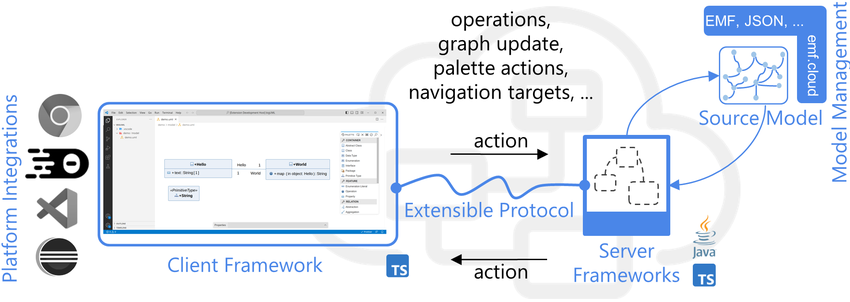
\includegraphics[width=\textwidth]{figures/glsp-overview.png}
	\caption[Overview of GLSP components]{Overview of GLSP components and their interplay. Taken from \cite{bork_vision_2024}.}
    \label{fig:glsp-overview}
\end{figure}

% ----------------------------------------------------------
\subsection{The Graphical Model Transformation Workflow}
\label{subsec:glsp_transformation}
% ----------------------------------------------------------

The architecture of GLSP rests on a two-model abstraction.
The \textit{Source Model} serves as the persistent source of truth and may itself be split into separate domain and notation concerns.
For example, the Eclipse Modeling Framework (EMF) can manage semantic logic independently of visual metadata such as node positions and element dimensions~\cite{metin_developing_2023}.
From the source model, the server derives the \textit{Graphical Model} (GModel), a typed and attributed graph that describes the diagram's structure and geometry.
It serves as the transient artifact exchanged with the client~\cite{bork_vision_2024}.
The natural interaction flow commences by the client encapsulating a user action and sending it to the server for validation and execution rather than applying it as a direct model edit~\cite{bork_vision_2024}.
The server processes the request, potentially modifies the source model, transforms the updated state into a new GModel, and returns it to the client.
The incoming GModel is then rendered as SVG.
This division also reflects a clear authority split: the server determines which elements are rendered based on domain state, while the client controls how they appear through CSS and SVG styling.
For trivial operations such as dragging, the client may apply immediate visual feedback optimistically, with final state reconciliation reserved for the server.
A practical advantage of this architecture is cross-runtime interoperability: a Java-based server can communicate seamlessly with a TypeScript client, allowing complex semantic logic to run on the Java Virtual Machine (JVM) while the user interface remains a responsive web application~\cite{metin_developing_2023, noauthor_eclipse-glspglsp-examples_2026}.